\section{配置期行和缓存：把不随样本变化的加法移出转换路径}
\label{sec:row-cache}
P7 实测的 LUT 退化促使本轮重新选择优化对象。对于同一个生效配置 epoch，
物理系数不变，只有活跃 slice 集合与开关状态变化。因此可以把
\(H_s=\sum_u W_{s,u}\) 缓存在系数装载器中，转换时只计算
\begin{equation}
T=\sum_s A_s H_s,\qquad
G=T-M,\qquad R=T-2W_{on}+R_d.
\end{equation}
其中 \(A_s\) 是物理行是否活跃的位图，\(M\) 和 \(R_d\) 仍按实际采样轨求和。
这不是拟合算法，也不是论文披露的新电路；它是当前可编程整数校正接口的精确工程变换。
本节描述行和缓存候选。其本地22项功能回归已完成，双版本定向与负控证据见本节末；
最终PPA取舍仍须由同约束综合及实际实现结果决定。

\begin{figure}[H]\centering
\begin{tikzpicture}[node distance=8mm and 10mm,box/.style={draw,rounded corners,align=center,minimum height=12mm,fill=blue!6},arr/.style={-{Latex[length=2mm]}}]
\node[box,minimum width=37mm] (write) {接受的配置写\\地址 $(s,u)$ 与新值};
\node[box,right=of write,minimum width=44mm] (delta) {$H_s-W_{s,u}+W_{new}$\\精确替换更新};
\node[box,right=of delta,minimum width=35mm] (cache) {18 行缓存\\每行54 bit};
\node[box,below=of write,minimum width=37mm] (store) {原物理系数表\\合法值47 bit};
\node[box,below=of cache,minimum width=35mm] (sum) {活跃位图门控\\18 行归约得到 $T$};
\draw[arr](write)--(delta);\draw[arr](delta)--(cache);
\draw[arr](write)--(store);\draw[arr](store.east)-|(delta.south);
\draw[arr](cache)--(sum);
\end{tikzpicture}
\caption{候选行和缓存的工程结构示意。系数与缓存只在同一个接受写边沿更新；这是结构说明，不是仿真波形。}
\end{figure}

\subsection{逐拍不变量与 clear 的语义}
必须证明的状态关系是每个周期都满足 \(H_s=\sum_u W_{s,u}\)，
而不是仅在完整装载结束时偶然相等。复位同时令系数和行和为零。
合法接受对 \((s,u)\) 的写入时，旧值先被减去，再加新值，系数和缓存同沿提交；
其余行不变。被拒写、运行锁定和空闲周期保持二者。
\code{clear_load} 只清除本 epoch 的 written bitmap，保留系数数值，因而也必须保留行和。
clear 之后的第一次重写仍然减去保留的旧值；若把 written=0 当成“旧系数为零”，
第二个装载 epoch 就会重复累计。这是定向负控应能识别的关键故障。

活跃行由物理 ID 的 OR 位图形成。重复 ID 会报警，但数值求和仍只包含该物理行一次；
缓存实现必须保持这一原有语义，不能改为每个逻辑槽重复累加。
无效 ID 不激活任何物理行。采样 dither 的列树继续读原物理叶子，
只移除 total 树的上层加法，不能连带删除列树仍需使用的叶值。

\subsection{宽度、资源预算和配置路径的代价}
合法写入满足 \(0<W<2^{47}\)。对一行 \(U\) 个单元，
\begin{equation}
0\leq H_s < U2^{47}\leq 2^{47+\lceil\log_2 U\rceil}.
\end{equation}
生产配置 \(U=71\) 因而需要54 bit，18行共972个候选状态位。
模块支持的最大 \(U=128\) 仍满足54 bit上界；\(U=1\) 时47 bit即可。
向原64-bit归约接口补零不会改变精度。按该上界作归纳，每次减旧值无下溢，
加新值后不越出行和宽度；此证明依赖装载器的合法写守卫，不适用于任意未经检查的外部位型。

原1278个有效叶的 total 归约需要1277次非平凡加法，
18行归约需要17次，源结构减少1260次加法。
on 树和 dither 列树保留；宽系数并行读也仍存在，不能由此宣称已转换成SRAM结构。
初版新增代价包括972个状态位、被选行和的读选择、旧系数读选择、一次减法和一次加法。
初版通过装载器的 \code{selected_weight} 显式共用写替换与配置读回的旧值路径，
避免只依赖跨层级优化来合并两个宽选择器；实际布线随后揭示这条全局反馈路径过长，
因此下面另检验逐物理行局部更新候选。

配置路径仍在同一个时钟域内，每次合法写必须满足真实 setup/hold。
不能因为软件通常慢速写寄存器，就把这条路径设为 false path 或多周期。
如果最终关键路径转移到“选择旧权重—减法—加法—行和寄存器”，
应在保留当前握手语义的前提下继续处理，或者报告实际可用频率。
本候选不增加转换流水级；P5/P6/P7 的15/13/11拍与16拍启动间隔仍须实测复核。

针对首次P5实际布线时出现的全局旧系数读回路径，又冻结了仅修改
\code{weight\_store.sv}的逐物理行局部更新候选：每个slice在本地选旧系数，
对本行执行\(H_s-W_{s,u}+W_{new}\)，并仅在被接受且地址命中时提交。
它避免先汇合成一条全局旧系数再反馈到任意行，却可能复制18组减加电路；
所以不能仅凭更短的逻辑连线推断PPA收益。
此候选RTL内容摘要为\code{6b27c64df11838428e7f364ac165c5986b51be586fd8cca1722d8095e54e7a22}。
官方Verilator 5.020下22项回归与三种生产lint通过；18-slice顶层P5/P6/P7
各有三模式、438个输出、7,680个协议周期和438个延迟观测，分别为15/13/11拍。
逐项原始日志与哈希见\code{docs/evidence/20260930/local\_row\_trial\_rtl/}。
这些仅是零延迟功能结果。后述同约束综合发现其LUT增加14.66\%，
实际路由又因拥塞等级7失败，故\emph{不保留}这个逐行独立读选的版本；
图中的功能通过不能抵消物理不可布通。

\begin{figure}[H]\centering
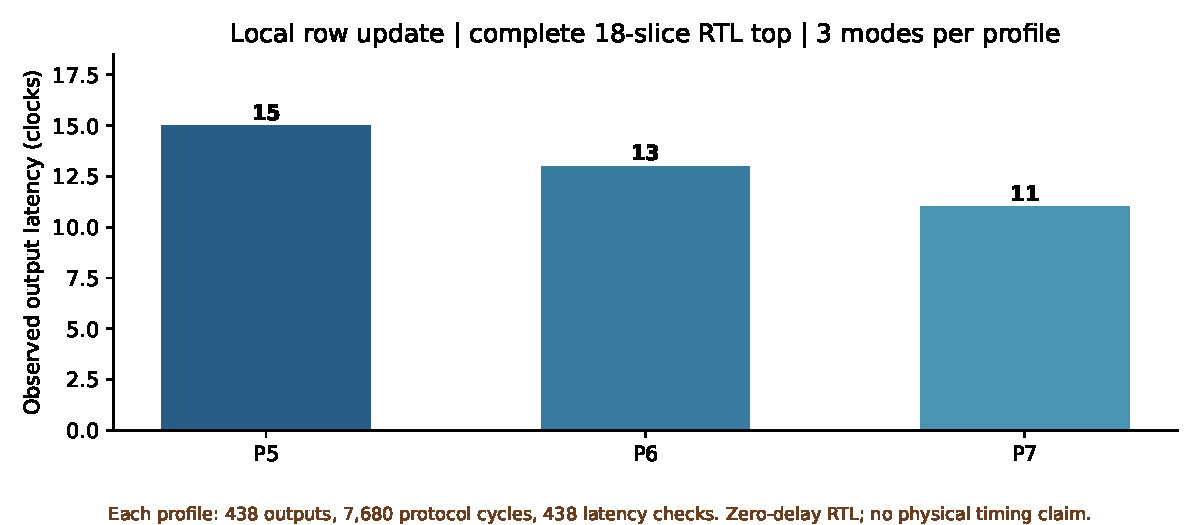
\includegraphics[width=0.84\textwidth]{figures/local_row_profiles.pdf}
\caption{局部行更新候选的实际RTL完整顶层输出延迟。三档结构的输出、周期和延迟检查数均从冻结日志重绘；脚本在作图前核对57项证据文件哈希，见\code{audit_figures/make_local_row_profiles.py}与同名\code{*.sha256.json}。柱高是数字时钟拍数，不能读作纳秒时序。}
\label{fig:local-row-profiles}
\end{figure}

\subsection{如何判定候选可以进入最终版本}
功能门禁要同时覆盖新状态不变量与使用缓存的真实生产链路。
直接驱动 \code{w_rom} 的叶模块保留常量参数关闭缓存的接口；
生产顶层开启缓存，两条路径均有独立标量参考。
定向验证应包含完整最大值行、同址连续替换、clear后重装、拒写、
32\(\times\)128边界、重复与无效ID，以及蓄意损坏一个缓存项后的失败见证。
完整结构顶层还须覆盖18个slice、三种dither模式、配置读回及 epoch 取消。

PPA门禁必须与精简P5采用相同25\,ns约束、器件和工具。
只报源码运算符削减，或只通过缓存关闭分支的回归，都不能算这一候选成功。
即使综合资源下降，仍须实际布局布线检查 setup、hold、pulse width、约束覆盖和DRC，
并对最终完整综合网表执行功能比较。

% Candidate-only evidence; root decides the final insertion point.
\subsection{行和缓存候选的双版本数值证据}
\label{sec:row-cache-evidence}
本节对应候选 RTL 内容摘要 \code{1e3fab94b7b2}\ldots，包含 26 项生产 RTL 文件；父提交为 \code{f028ec5}。
来源为 \code{docs/evidence/20260930/row_cache/}，属于新的本地功能验收，不能移用父提交 CI 的通过结论。
归档中的 Verilator 5.020 与运行时标识为 5.49 的开发版，分别完成相同的五种加载器几何和七种归约器几何。
每个版本的 16,150 个加载事务步与 1,430,848 个归约输入样本按各自单位列示，不相加为覆盖率。
5.020 的附加复验只包括这两项，不能据此声称该工具本地重跑了全部 22 个 bench。

最大装载先把整张表写为 \(W_{\max}=2^{47}-1\)，故每个含 \(U\) 项的物理行应为 \(U W_{\max}\)。
\code{clear_load} 清除完整性位图，保留权重与行和；随后将行 0 的一个旧最大权重替换为 1，
独立期望成为 \mbox{\((U-1)W_{\max}+1\)}。图\ref{fig:row-cache-evidence}分别保留原日志的 \code{row_last} 与 \code{row0} 标签。
制图器以 Python 任意精度整数重新计算，不把超过 \(2^{53}\) 的行和先转为浮点数再判断相等。
全部十个阶段观测在两个版本原始日志中逐条匹配；归档没有单独记录 clear 当拍的数值，因而不额外绘制该时刻。

\begin{figure}[H]\centering
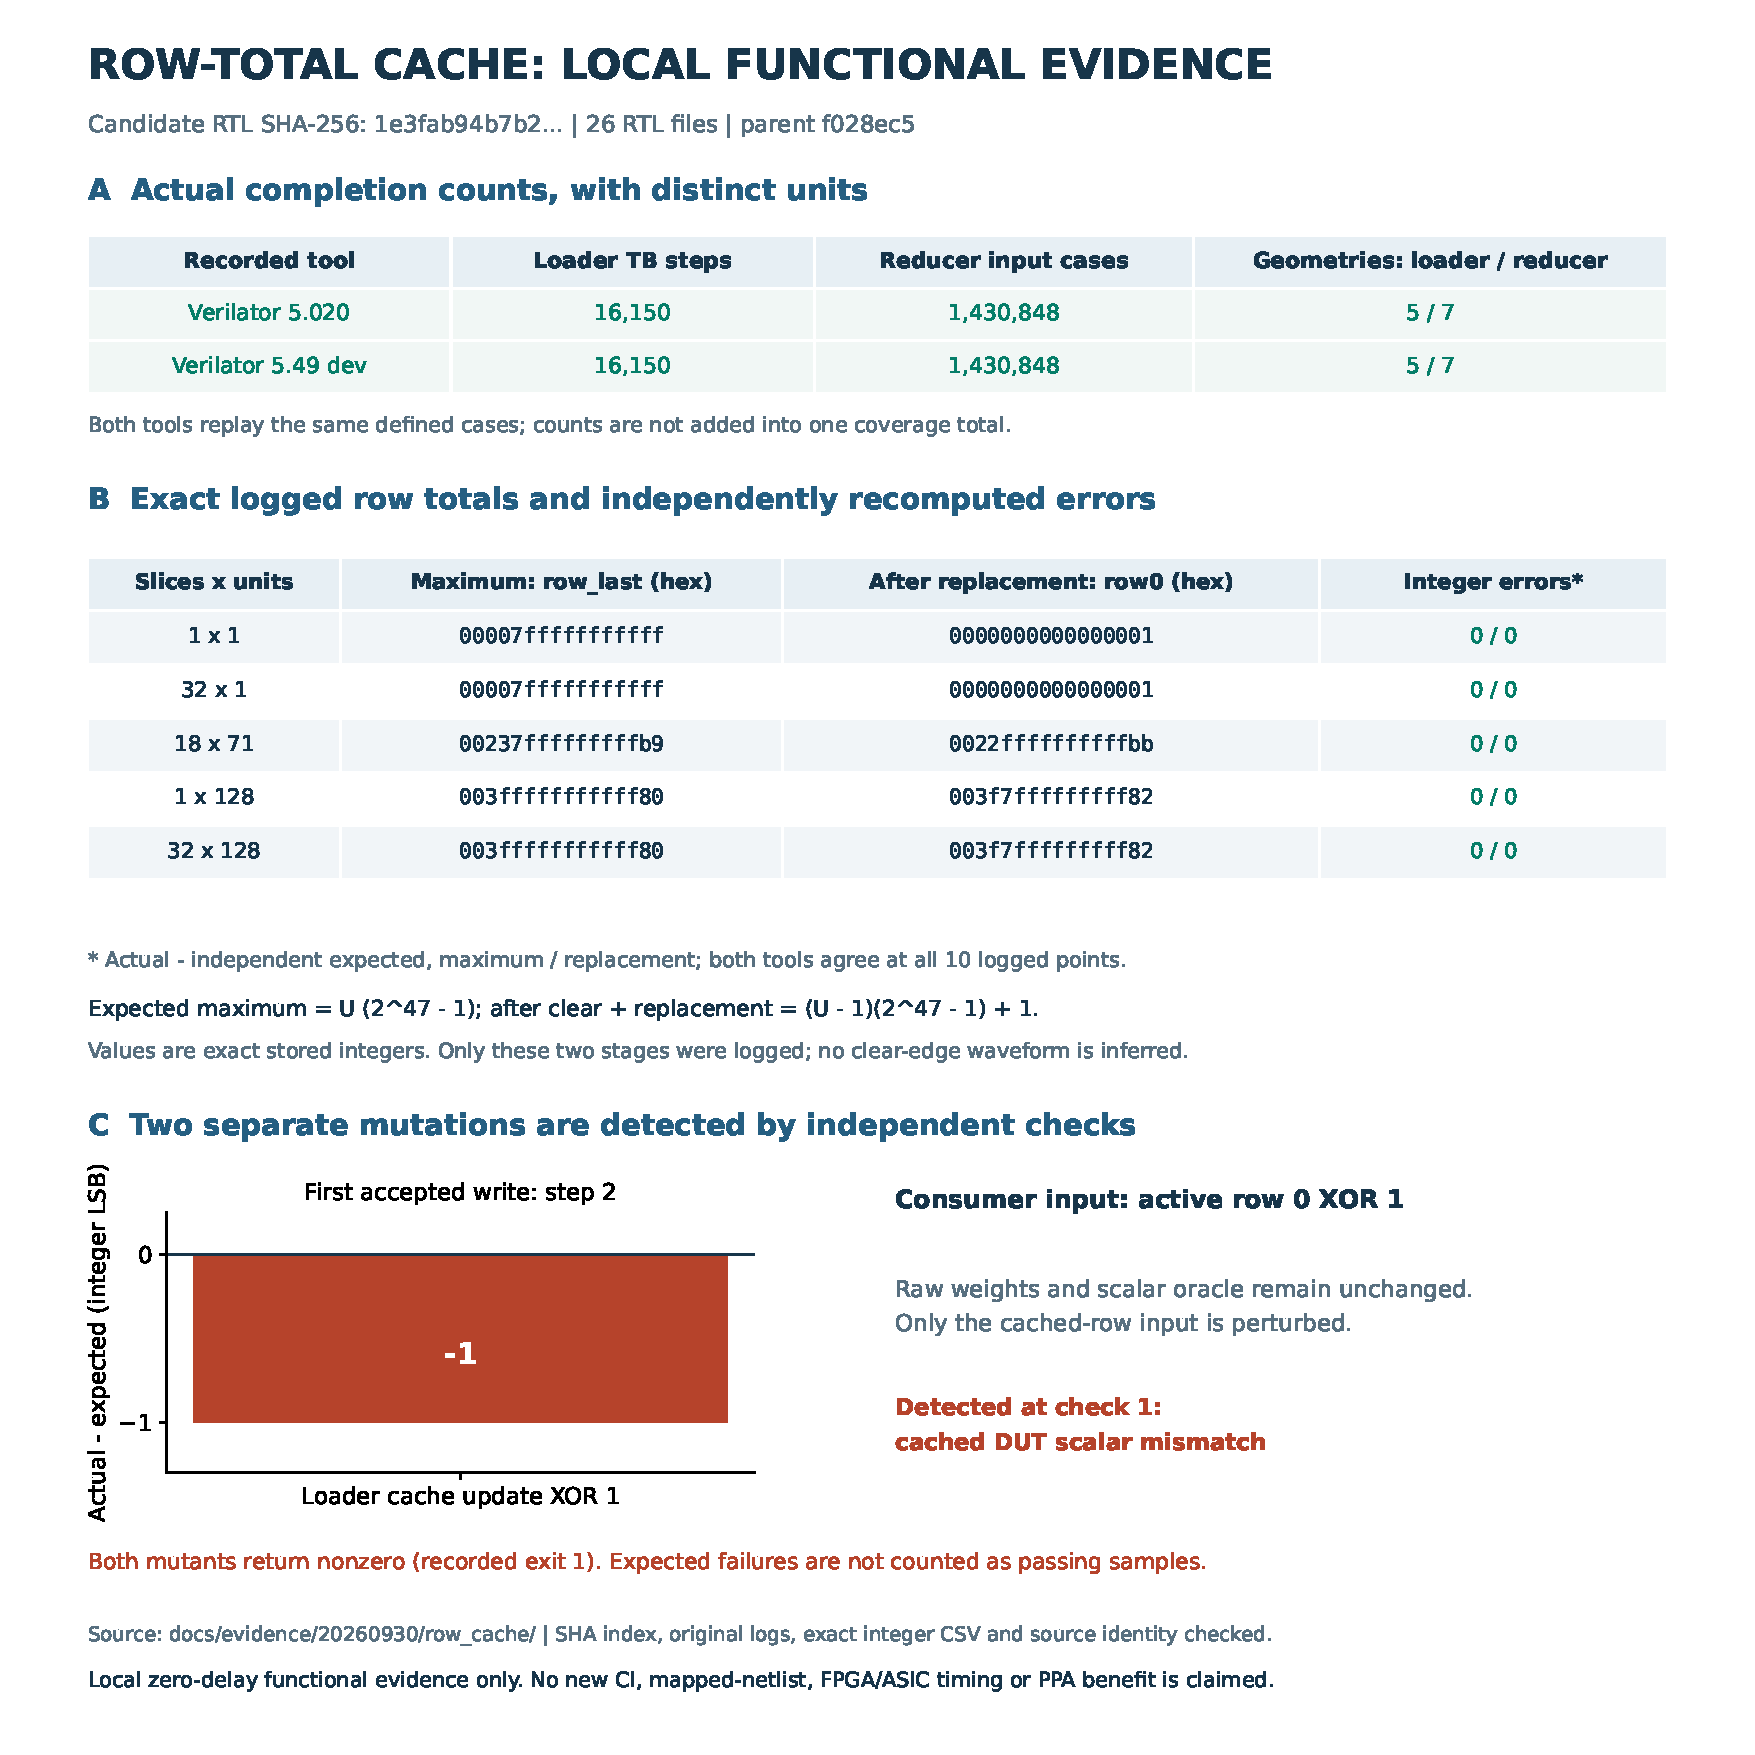
\includegraphics[width=\textwidth]{figures/41_row_cache_evidence.pdf}
\caption{候选行和缓存的真实日志证据。上表为双版本完成计数；中表为五种几何在最大装载和 clear 后替换两个已记录阶段的精确十六进制整数，独立整数公式的误差均为零。下方展示两个分别注入的错误被检出；没有由完成标记推造波形，也没有将功能通过解释为 PPA 收益。}
\label{fig:row-cache-evidence}
\end{figure}

两个负控分别检查生产者和消费者。
第一项只翻转行和写回结果的最低位，在首次接受写的第 2 步出现实际值相对独立期望少 1，加载器检查立即失败。
第二项只翻转活动行 0 的缓存输入最低位，原始权重、未缓存实现、旧公式和 scalar oracle 都不变；
第 1 个比较样本触发 \code{cached DUT scalar mismatch}。
后者排除了“缓存输入被忽略而仍通过普通数值回归”的假阳性；它不是新功能正常输出的样本。

可复现入口为 \code{audit_figures/make_row_cache_evidence.py}，来源清单为 \code{audit_figures/41_source_hashes.json}。
脚本校验归档 SHA、26 项 RTL 摘要、完成计数、十个实测值以及两份负控的失败日志与源文件摘要。
这些结果说明行和维护与消费在所测功能条件下符合独立判据；缓存候选的实际资源、物理建立/保持时序及 ASIC 目标频率仍应由同一候选的后续综合和实现报告单独判定。

